\chapter{Physical Database Design}

The design of a relational database has four phases:
\begin{itemize}
    \item Requirements analysis, for the specification of data to be taken into account and the services to be implemented;
    \item Conceptual design, defining the representation of the entities of interest and their properties, associations, and integrity constraints;
    \item Logical design, defining the logical schema;
    \item \textbf{Physical design}, defining the appropriate storage structures used for the DBMS in order to guarantee the desired performances.
\end{itemize}
The information needed in order to work on the physical design of a database are:
\begin{itemize}
    \item \textbf{Statistics}: information about number of records in each relation, record size, number of pages used, distinct values per attribute, maximum and minimum values, and a distribution (if not uniform);
    \item \textbf{Workload description}: a description of critical queries and updates and their frequency, along with their respective expected performances. 
    For each critical query, this description specifies the relations and attributes used, the attributes used in selection and join conditions, and the selectivity factor of conditions. For updates, it also specifies the type (INSERT/DELETE/UPDATE).
    
    This information is usually represented using \textbf{ISUD} (Insert, Select, Update, Delete) tables: for each application, they specify the execution frequency, the percentage of data used, and the type of operation;
    \item \textbf{Knowledge about the DBMS}: data organizations, indexes, and query processing techniques supported.
\end{itemize}
Once this information is known, decisions can be made for storage structures and indexes.

\section{Database Design}

\subsection{Storage Structures}

For the storage structures, a solution can be selected from the ones seen in the first chapter: sequential, heap, hash, or index organization. Heap organization is best for small databases where insertions are more frequent than searches, sequential organization is best if it's interesting to keep static data sorted on a key, hash organization is best if the most common operation is record search by a key, and finally index organizations can both keep data sorted on a key and support efficient equality and range searches.

\subsection{Indexes}
The main goal of indexes is to avoid a relation scan when few records are looked for. Systems will usually automatically define indexes on primary and secondary keys. They can speed up searches, but they occupy memory and can slow down updates of the attributes on which they are defined, since any change to the actual records must be reflected in the index as well. In general, indexes are unnecessary for relations that occupy very few pages, or for attributes that are not very selective. The problem of selecting useful indexes does not have a trivial solution, due to the large number of possibilities, which is why most commercial systems provide tools to assist in the resolution. In the absence of such tools, we must consider which are the critical queries and which plan the optimizer chooses for them, evaluating whether an index may improve performances.

For example, we should consider defining indexes on  attributes used in queries that require sorting (OrderBy, GroupBy, Distinct, Set operations); on selective attributes in the WHERE clause, choosing the appropriate structure depending on the type of search (equality, range, multi-attribute); to improve joins with IndexNestedLoop. Indexes can be defined for single queries (local view) or for workloads (global view).

An index $I$ is unnecessary if it is \textbf{subsumed} by another $I_2$, meaning that the attributes of $I_1$ are included as prefix within those of $I_2$. For example, an index on a single attribute $A$ is subsumed by an index on $(A, B)$, and both are subsumed by an index on $(A, B, C)$.

Two indexes supporting two queries can be \textbf{merged} together into one index supporting both queries. For example, if two queries caused the creation of indexes on $(A, B)$ and $(A, C)$, respectively, they can be merged into $(A, C, B)$.

From the global viewpoint, a way to create indexes is to start by defining useful indexes on single critical queries; then, indexes that can be subsumed are removed from the set of all indexes, and the benefit/cost ratio is evaluated for the remaining ones.

\paragraph{Use of Clustered Indexes} Clustered indexes are best used for equality and range searches on non-key attributes, even if the selectivity factor is not very restrictive. It can also be useful for queries in which data must be sorted (usually when the query has a GroupBy).

\paragraph{Multi-Attribute Indexes} Indexes defined on multiple attributes at once can be used for queries with equality-equality searches, or equality-range searches. It's important to consider the order in which the index attributes are specified: the first one should be the one used for mostly equality searches.

Since each element in the index contains several attributes, there is a greater chance that the optimizer will generate plans using only the index. However, multi-attribute indexes must be updated each time an update is done on an attribute on which it is defined, and occupies more memory than an index on a single attribute.

\paragraph{Indexes for Join} Clustered indexes on a non-key join attribute of the internal table can improve the performances of an IndexNestedLoop, since it requires an IndexFilter as its inner operand.

\paragraph{Index-Only Plans} In some cases, it is possible to execute Index-Only plans for a query, i.e., plans in which only indexes are accessed instead of the actual data. These plans can be generated if an index has been defined on the attributes appearing in the SELECT DISTINCT clause, or the GROUPBY clause.

Also, if indexes are defined for the inner operand on a foreign key needed for a join, the plan can use IndexOnlyFilter instead of IndexFilter.

\section{Database Tuning}

Database tuning includes all activities carried out to meet requirements regarding the performance of database applications. By ``performance'', we refer to runtime performance, so \textbf{throughput} (number of operations completed in a unit of time), \textbf{response time} (time to execute an application), and \textbf{resource consumption} (temporary or permanent memory used). For each potential decision to be taken, the trade-off between its costs and benefits is evaluated. Costs include any monetary cost (hardware, software), working hours, technical costs, while benefits include any improvement in performances (sometimes quantified in monetary effects, although often not easy to do). \\
Tuning considers the following aspects:
\begin{itemize}
    \item Applications: user queries and transactions;
    \item DBMS: configurations, parameters, database schema, storage structures;
    \item Operating system: system parameters and configuration for I/O, network communication;
    \item Hardware: components used for CPU, main and permanent memory.
\end{itemize}
A basic idea at the basis of database tuning is Pareto principle: by applying 20\% of the effort one can achieve 80\% of the desired effects, meaning that a fully optimized system may be unnecessary, and the process should instead focus on smaller (but with significant improvements) changes.
\begin{figure}[h]
    \centering
    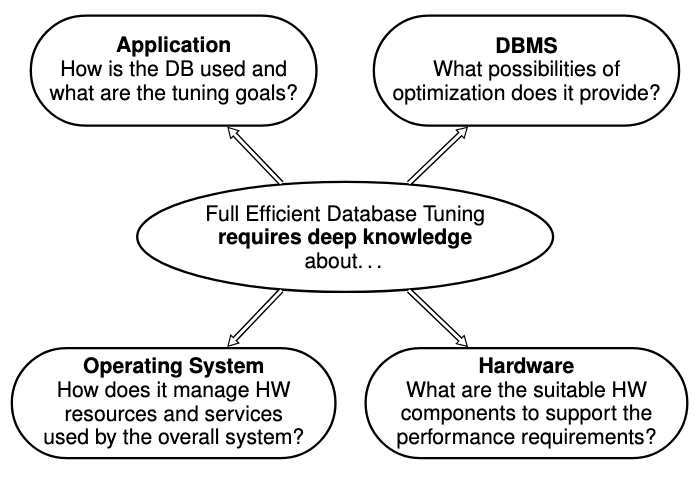
\includegraphics[width=0.5\linewidth]{img/quadrilemma.png}
    \caption{The DBMS tuning \textit{quadrilemma}.}
    \label{fig:quadrilemma}
\end{figure}
This is a complex and continuous process which involves different professional figures:
\begin{itemize}
    \item Database and applications designers, who have knowledge about applications and the DBMS, but may have little knowledge about OS or hardware;
    \item Database administrators, who have good knowledge about DBMS, OS, and hardware, and may have little knowledge about applications;
    \item Database experts, who usually have strong knowledge in DBMS, OS, and hardware, but very limited knowledge about applications.
\end{itemize}

\subsection{Index Tuning}

The initial choice of indexes could be revised for different reasons: the workload of the database may reveal that some queries initially considered critical are not actually executed that often, while others which had initially been thought of as infrequent turned out to be important. In some cases, the optimizer does not generate the physical plan that was expected. Either way, changing indexes can improve performances.

\subsection{Query Tuning}

If the optimizer does not transform SQL queries, they can be explicitly rewritten with two set of rules:
\paragraph{Semantically Equivalent Rewriting}
\begin{itemize}
    \item If a query has an Or condition, it may be rewritten using an Union of different queries, or using the In predicate specifying both conditions;

    \item If a query has an And of different predicates, it can be rewritten as a condition with Between (if the values in the predicates describe a range);

    \item Avoid arithmetic expressions on attributes used in conditions (e.g., instead of writing ``Salary*2 = 100'', write ``Salary = 50'', because for the first condition the optimizer may not use an index);

    \item Subqueries can be rewritten as joins;

    \item Avoid temporary views. If the optimizer cannot rewrite the query without views, the physical plan will have an higher cost;

    \item Redundant Having and GroupBy should be removed.
\end{itemize}

\paragraph{Semantically Non-Equivalent Rewriting}
\begin{itemize}
    \item Avoid useless Distinct and OrderBy clauses;
    
    \item Avoid cartesian products.
\end{itemize}

\subsection{Transaction Tuning}

Another cause of inefficiency in DBMS is the way transactions are programmed. They should be as short as possible to reduce the duration of the locks they hold over data objects (although as seen before many modern systems use more sophisticated locks instead of read-write locks, so this problem is not as big), and they should not block data during database loading and during read-only transactions. Complex transactions should be split into smaller ones. Also, if a transaction has to stop because user input is being asked, it should commit and restart after input has been received. Each transaction should have the appropriate block granularity (record, page, table, etc.), as well as the appropriate isolation level:
\begin{itemize}
    \item \textbf{READ UNCOMMITTED}: the reads of records are performed without requesting any locks, so dirty reads are possible;

    \item \textbf{READ COMMITTED}: the transaction obtains locks on records, released right after reading, and exclusive locks before writing (held until the end). This prevents dirty reads but not non-repeatable reads.

    \item \textbf{REPEATABLE READ}: the transaction holds both read and write locks on records released at the end. This avoids     \item \textbf{READ COMMITTED}: the transaction obtains locks on records, released right after reading, and exclusive locks before writing (held until the end). This prevents dirty reads but not non-repeatable reads, but introduces the problem o \textbf{phantom records}: for example, if a transaction reads a set of records from a table which satisfy a condition $\psi$, and right after a second transaction writes a new set of records in that table with also satisfy $\psi$, the first transaction will never see those new records.

    \item \textbf{SERIALIZABLE}: the default isolation level, where read and write locks are of different sizes. Any read lock on a table will be in conflict with any update. It avoids all problems seen before, but reduces the number of concurrent transactions executable per unit of time.
\end{itemize}
Commercial DBMS don't necessarily provide all previous levels of isolation, or may have different default levels. Also, some of them provide the SNAPSHOT isolation level.

\subsection{Logical Schema Tuning}

If the physical design is not able to provide adequate performances, it may be necessary to modify the logical schema, using two types of restructuring: \textbf{partitioning} and \textbf{denormalization}.

\paragraph{Partitioning}

Partitioning can be either vertical or horizontal.

\textbf{Vertical partitioning} reduces the volume of data transferred from/to permanent memory and cache, splitting a relation separating its attributes into two sets, such that one set should contain the most frequently accessed attributes. Each partition will still have the primary key of the original relation as a subset of its attributes.

\textbf{Horizontal partitioning} reduces the cost of accessing a large relation by splitting it into sets of records, separating frequently accessed records from the others. Each partition will have all the original attributes of a disjoint subset of the original records.

\paragraph{Denormalization}

Normalization is the process of decomposing a table into smaller ones to reduce redundancy; denormalization is the opposite, so the process of adding columns to tables to improve the performance of read-only queries. This is useful when two or more tables are often read after joins, so instead of having to compute it every time, their information can be stored together in a single table.

\section{DBMS tuning}

If all else fails, the database system must be tuned. The most important things to consider can be divided into three levels that interact with each other:
\begin{itemize}
    \item \textbf{Transaction Management}: intervening on parameters such as log storage, frequency of checkpoints and dumps, etc. The more frequent they are, the faster the database can be fully restarted after a system failure or disaster, but the system performances also degrade, since they subtract resources from normal activity;

    \item \textbf{Database Buffer Size}: if the buffer is larger, performance of application improves, but it shouldn't be so big id does not fit in main memory;

    \item \textbf{Disk Management}: adding disks or using RAIS systems if disk I/O is a bottleneck, adding more memory, or using a faster processor;

    \item \textbf{Parallel Architectures}: this is an issue that strictly depends on the system in use.
\end{itemize}
An alternative is database \textbf{self-tuning}.